

\chapter{Distributed GPU SpMV}
\label{chap:multigpu_rbffd}

%%%%%%%%%%

%DONE: extending work from chapter 6 we return to the GPU but this time attempt to span multiple GPUs
%TODO: describe context with multiple devices, we assume one device per context
%TODO: describe multiple queues, assume two for SpMV (why? indep operation, overlapping kernel execution not just comm)
%TODO: nonoverlapping test case description
%TODO: overlapping test case description
%TODO: benchmark nonoverlapping shows significant loss on multiple GPUs one host
%TODO: Known issue on Cascade is that all GPUs are attached to the same I/O hub
%TODO: limits performance because transfers to each GPU are serialized 
%TODO: we have explicit barrier on comm ensuring that each kernel gets to transfer at the same time
%TODO: benchmark overlapping shows 5x boost because queues do not necessarily transfer at the same time
%TODO: also the multiple queues ensure overlapping memtransfer and some comp with the original spmv. 
%TODO: a single queue would have synchronous copy following kernel execution and synchronous SpMV if both in same queue
%TODO: two queues allows asynchronous copy and overlap between SpMVs.

%TODO: cuda mpi aware


Today, high performance computing centers around the world are leveraging GPU accelerators to reach their peak performance. For example, the Titan supercomputer at Oak Ridge National Lab is (as of this writing) ranked \#2 on the world-wide Top500 list, and achieved that spot with a total of 18,688 NVidia K20 GPUs and 18,688 AMD Opteron CPUs in a 1:1 pairing for a theoretical peak of 27.1 PFLOP/sec \cite{TitanGPUCluster}. 
In some cases, HPC installations like the Keeneland project \cite{Vetter2011} boast significantly more GPU accelerators than CPU counterparts. The Keeneland Full-Scale (KFS) system has 528 Intel Sandy-Bridge CPUs and 792 NVidia Fermi-class GPUs in 264 compute nodes (i.e., 2:3 CPUs:GPUs), and a theoretical peak of 615 TFLOP/sec \cite{Vetter2011}. 

Ultimately, finding a way to harness the tera- and peta-scale performance from such clusters is a grand challenge for our work on RBF-FD and other RBF PDE methods. To this end, we present a multi-GPU implementation of RBF-FD.

In Chapter~\ref{chap:gpu_rbffd}, we have already developed two different approaches to computing RBF-FD on a single GPU: the first using custom OpenCL kernels for RK4 time-steps, and the second using ViennaCL for the same tasks. Then in Chapter~\ref{chap:distributed_rbffd}, we laid the foundation for a distributed RBF-FD that spans the nodes of an HPC cluster, and demonstrated scaling up to 1024 processors (128 nodes). This chapter combines those algorithms to produce the first (to our knowledge) multi-GPU implementation of the RBF-FD method with overlapping communication and computation. 

One issue with distributing computation across multiple GPUs is that the GPUs excel at accelerating computation, but do nothing to reduce the cost of communication. With communication latency suddenly disproportionately large compared to computation, the distributed GPU implementation loses its ability to scale well. As part of this chapter, we detail an algorithm to hide communication latency behind overlapped computation. The algorithm presented herein is an organic extension to the overlapping communication and computation algorithm in Chapter~\ref{chap:distributed_rbffd}. 

Our multi-GPU implementation leverages non-blocking MPI communication plus two asynchronous OpenCL queues to amortize the cost of data transfer between CPU and GPU, MPI communication, and in some cases hide some computation. 

%With the popularity of GPU clusters, there are naturally a number of related investigations in the literature that consider overlapping communication and computation for multi-GPU applications. For example, Kim and Park overlap communication and computation in their implementation of a Finite-Difference Time-Domain algorithm and demonstrate near perfect strong scaling up to 6 GPUs \cite{KimPark2012}. \cite{Thibault2009}
%
%TODO: \cite{Goeddeke2009} \cite{Erez2007}
%Similar approaches to overlapping communication and computation can be found in \cite{Schubert2011} and \cite{Thibault2009}.

%Lawlor \cite{Lawlor2009} wraps a subset of MPI collectives, memory copies between GPU and CPU, and---to some extent---callbacks to GPU kernels behind a simplified API called cudaMPI. Although the concept of cudaMPI is good for minimally invasive design, the library only provides a handful of  a limited subset of MPI  a for overlapping communication and computation.  


\section{Multi-GPU RBF-FD}

In order to develop the multi-GPU implementation, we return to the idealized test case proposed in Chapter~\ref{chap:distributed_rbffd}: four derivatives on a 3-D regular grid are computed via SpMV and used as the intermediate vectors for an RK4 time-step. At the end of each SpMV a communication collective synchronizes external dependencies for each subdomain.

In Chapter~\ref{chap:distributed_rbffd}, the SpMV was assumed run on the CPU. Herein, it is assumed to be computed via one of the GPU algorithms presented in Chapter~\ref{chap:gpu_rbffd}. For now the actual choice between custom OpenCL kernels and ViennaCL does not matter. Later, when we consider the scaling of this algorithm, the ViennaCL implementation is assumed. 

Our original attempt at multi-GPU RBF-FD, described in \cite{BolligFlyerErlebacher2012}, utilized blocking communication (i.e., \texttt{MPI\_Send}/\texttt{MPI\_Recv}) for synchronization. The blocking communication functioned for debugging purposes, but was not practical. In Appendix~\ref{app:keeneland_alltoallv_benchmarks}, we provide supplementary data that demonstrates the result of replacing the blocking send and receives with an \texttt{MPI\_Alltoallv} (i.e., the GPU equivalent of Figure~\ref{fig:alltoallv_cpu}). In both cases the SpMV is a single kernel launch and the synchronization includes both an encode and decode phase (see \S~\ref{sec:local_ordering}). 

The two multi-GPU algorithms that follow build off of Figure~\ref{fig:no_decode_cpu} and Figure~\ref{fig:overlap_cpu}; the final collectives tested in \S~\ref{sec:mpi_improvements}. 
When operating on multiple GPUs we avoid the copy-out or decode phase by requiring that the local ordering of nodes sort the set $\setDepend$ by the rank of the process sending each node. This way, when the MPI collective finishes and all values arrive contiguous by provider, the data can be copied directly to the GPU without reordering.

\subsection{Non-overlapped Algorithm}

Figure~\ref{fig:isendirecv_gpu} illustrates the GPU accelerated equivalent of Figure~\ref{fig:no_decode_cpu} with \texttt{MPI\_Isend}/\texttt{MPI\_Irecv} communication. In this case the communication has no overlap with computation of the SpMV. 

The algorithm for Figure~\ref{fig:isendirecv_gpu} is as follows. First, the CPU launches \texttt{MPI\_Irecv} as soon as possible. When control returns from the non-blocking launch, the CPU queues a blocking memory transfer to copy $\mathcal{O}$ from the GPU down to the CPU. Once the transfer is complete the CPU encodes the send buffers and issues the non-blocking \texttt{MPI\_Isend}. An \texttt{MPI\_Waitall} blocks until $\mathcal{R}$ is received. The CPU then queues both a non-blocking memory transfer to copy $\mathcal{R}$ from CPU to the GPU, and the SpMV kernel launch for $\mathcal{Q}$ (i.e., the local subdomain). 

%This non-overlapping algorithm is presented in order capture 

\begin{figure} 
\centering
\begin{subfigure}{0.48\textwidth}
\centering
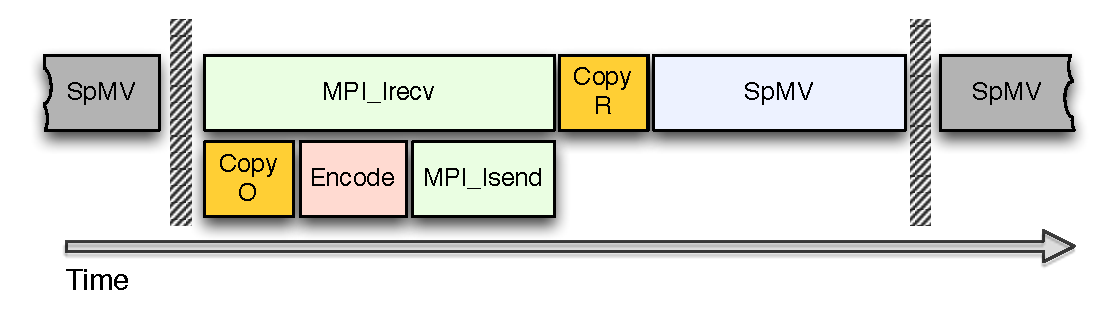
\includegraphics[width=\textwidth]{../figures/omnigraffle/GPU_IsendIrecv.pdf}
\caption{GPU and MPI\_Isend/MPI\_Irecv (Non-Overlapping)}
\label{fig:isendirecv_gpu}
\end{subfigure}
\quad
\begin{subfigure}{0.48\textwidth}
\centering
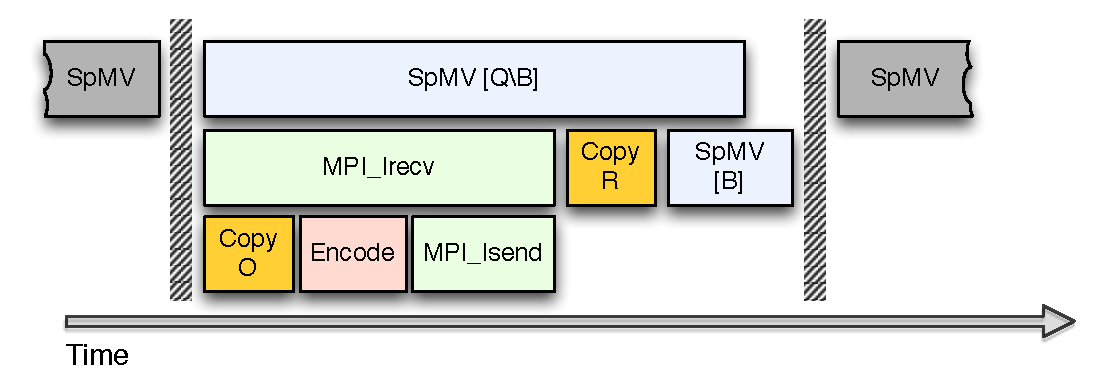
\includegraphics[width=\textwidth]{../figures/omnigraffle/GPU_OverlapGPU.pdf}
\caption{GPU and MPI\_Isend/MPI\_Irecv (Overlapping)}
\label{fig:overlap_gpu}
\end{subfigure}
\caption{Overlapping GPU kernels with CPU managed communication. Task block sizes are not drawn to scale.} 
\label{fig:gpu_mpi_tuning}
\end{figure}

\subsection{Overlapping with the GPU}

Our overlapping SpMV algorithm is illustrated in Figure~\ref{fig:overlap_gpu}. This algorithm utilizes two sets of asynchronous commands: 
\begin{itemize} 
\item \emph{Non-blocking MPI}. The \texttt{MPI\_Isend}/\texttt{MPI\_Irecv} routines are used to post communication and immediately return the control of computation to the main CPU thread. 
\item \emph{Asynchronous GPU Queues}. Two OpenCL queues (\cite{Gerstmann2009}) are constructed within the same context for a single GPU. Each queue allows commands (e.g., memory transfers and kernel launches) to be sent to the GPU independently. Fermi- and Kepler-class GPUs, which support concurrent kernel execution, overlap execution of the commands across multiple queues. Within each queue commands are processed sequentially.
\end{itemize}

The algorithm for Figure~\ref{fig:overlap_gpu} starts with the construction of two OpenCL queues, $Q_1$ and $Q_2$. Then, the algorithm first activates $Q_1$ and launches the SpMV for $\mathcal{Q} \backslash \mathcal{B}$ (i.e., nodes on the interior of the subdomain). The kernel launch returns immediately and the non-blocking call \texttt{MPI\_Irecv} is made. Next, the CPU activates $Q_2$ and issues the memory transfer on $\mathcal{O}$. The CPU flushes $Q_2$ to ensure the transfer of $\mathcal{O}$ is complete before it starts encoding MPI buffers. When \texttt{MPI\_Isend} is called, the CPU uses \texttt{MPI\_Waitall} to block until $\mathcal{R}$ is received. The CPU asynchronously issues the memory transfer for $\mathcal{R}$ on $Q_2$, followed by another asynchronous kernel launch for the SpMV on $\mathcal{B}$. Ideally, while all of this activity happens on $Q_2$ and in MPI, the SpMV on $Q_1$ continues processing. Since the SpMV on $Q_1$ may complete before the SpMV on $Q_2$, the CPU flushes $Q_1$. Once $Q_1$ is complete the kernel flushes $Q_2$ to complete the iteration. 

\section{Strong Scaling Performance}

We now demonstrate the performance of our multi-GPU algorithms. In all cases the strong scaling of the ViennaCL ELL GPU implementation is tested.  

%Appendix~\ref{app:keeneland_alltoallv_benchmarks} demonstrates scaling of our custom OpenCL kernels using the \texttt{MPI\_Alltoallv} collective. The data was generated on the Keeneland Initial Delivery (KID) system \cite{Vetter2011} and is provided for comparison with the original benchmarks in \cite{BolligFlyerErlebacher2012}. We tested the strong scaling of RBF-FD kernels up to 10 GPUs (1 GPU per compute node) for the small problem size of $N=27556$ nodes. Non-overlapping communication (\texttt{MPI\_Alltoallv}) synchronizes GPUs as they execute iterations of the RK4 time-scheme. The benchmarks on Keeneland tested

Chapter~\ref{chap:gpu_rbffd} introduced the Cascade cluster, which contains up to 32 NVidia M2070 GPUs, 8 NVidia K20 GPUs and 3 Intel Xeon Phis. Although Cascade is not a large GPU cluster like Titan or Keeneland, it suffices for prototyping GPU code, and performing simple scalability tests on the various hardware options. In the benchmarks that follow, we scale up 32 M2070 GPUs and measure the GFLOP/sec for the distributed SpMV applied to an ELL matrix with a total of $N=4096000$ rows and $n=17, 31, 50$ and $101$ nonzeros per row. GPUs are each paired with a unique MPI process on the CPU. 

Table~\ref{tbl:cascade_m2070_nonoverlap} presents three groups data (GFLOP/sec) observed for each $1, 2, 4$ and $8$ compute nodes. The first group tests the execution of one MPI process per node (i.e., 1 PPN) for each compute node. The second and third groups scale the number of processes per node two four GPUs respectively. Data for the $n=101$, single process, single node test case could not be executed due to the limited memory on the M2070 GPUs (i.e., 6 GB available and the ELL matrix alone requires $((2*N*n)*8\ \text{bytes}) = 6.6$ GB).

\begin{table}[htb]
\centering
\caption{GFLOP/sec achieved by the distributed ELL SpMV on Cascade's M2070 GPUs, with non-overlapping MPI communication. The SpMV computes derivatives over a 3-D regular grid of size $N=4096000$ nodes (i.e., $160^3$). Data reflects various combinations of stencil sizes, number of compute nodes and number of processes per node (PPN). GPUs are attached to each process per node (i.e. 4 PPN implies 4 GPUs). }
\label{tbl:cascade_m2070_nonoverlap}
\begin{tabular}{c|c|c|c|c|c|c}
 \multicolumn{2}{c}{ } & \multicolumn{4}{|c|}{Observed GFLOP/sec} \\  \hline
Compute Nodes &   PPN  &   n=17   &   n=31   &   n=50   &   n=101   \\ \hline
1  &  1  &  8.4  &  8.4  &  8.9  & --  \\
2  &  1  &  6.1  &  6.8  &  6.4  &  7.6 \\
4  &  1  &  6.9  &  9.1  &  10.3  &  13.3 \\
8  &  1  &  12.1  &  14.6  &  12.1  &  23.0 \\ \hline
1  &  2  &  3.4  &  4.1  &  3.7  &  4.2 \\
2  &  2  &  4.4  &  5.4  &  6.5  &  8.1 \\
4  &  2  &  11.1  &  9.3  &  9.9  &  14.2 \\
8  &  2  &  15.9  &  15.4  &  22.2  &  23.9 \\ \hline
1  &  4  &  3.3  &  4.4  &  5.1  &  5.5 \\
2  &  4  &  8.3  &  7.6  &  9.5  &  11.0 \\
4  &  4  &  12.4  &  12.9  &  18.7  &  18.0 \\
8  &  4  &  17.4  &  28.4  &  28.0  &  37.4 
\end{tabular} 
\end{table}

The data in Table~\ref{tbl:cascade_m2070_nonoverlap} shows that without overlapped communication and computation our multi-GPU scaling is poor in all cases. For 8 compute nodes and 1 PPN (i.e., 8 GPUs total) the code achieves only 18\% - 20\% strong scaling efficiency. When increased to multiple GPUs per node, we find that the performance actually decreases by as much as a factor of two. 

The reduced performance observed for multiple GPUs per node (e.g., 1 compute node, 4 PPN) reflects a known design flaw on Cascade illustrated in the block diagram in Figure~\ref{fig:cascade_iohub}. Each of the M2070 compute nodes on Cascade has four GPUs attached to an NVidia proprietary hub, which is in turn connected via PCI Express to the I/O Hub for the CPUs. The single lane connection between the I/O Hub and the NVidia Hub acts as a bottleneck when copying data to multiple GPUs. Simultaneous data transfers contend for access to the lane and transfers are serialized. Serializing the data transfers can effectively double or quadruple the run-time. 

\begin{figure}
\centering
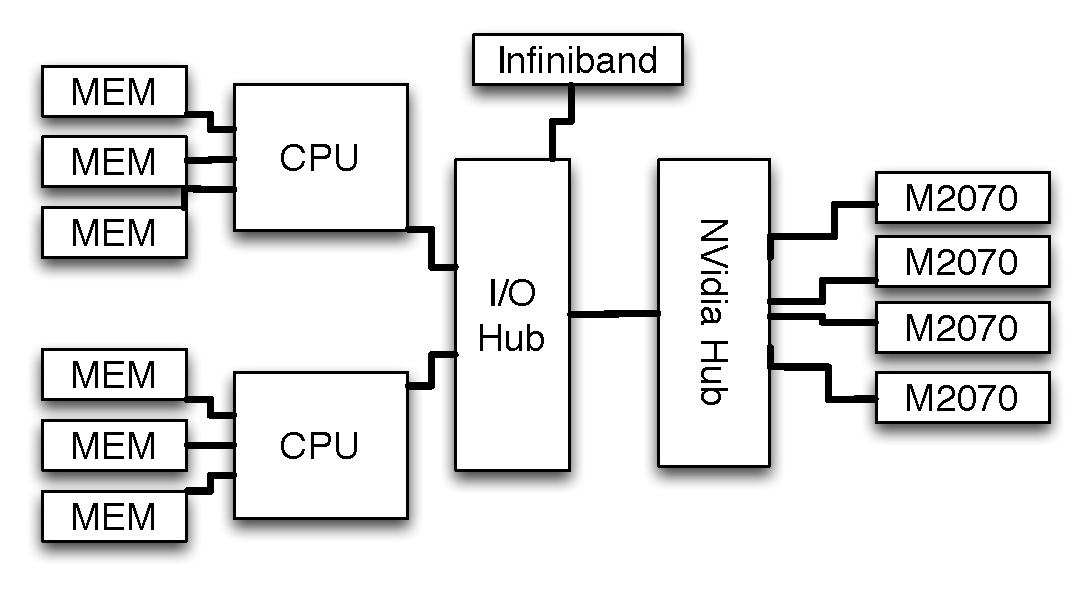
\includegraphics[width=0.5\textwidth]{gpu_content/omnigraffle/CascadeIOHub.pdf}
\caption{A block diagram of Cascade's hardware structure. While GPUs can operate independently, the single lane connecting the I/O Hub to the NVidia Hub acts as a bottleneck. Simultaneous memory transfers to multiple GPUs must serialized to cross the link. Structure based on the output from \texttt{lspci -tv}. }
\label{fig:cascade_iohub}
\end{figure}


\begin{table}[htb]
\centering
\caption{GFLOP/sec achieved by the distributed ELL SpMV on Cascade's M2070 GPUs, with MPI communication overlapping a split SpMV on the GPU. The SpMV computes derivatives over a 3-D regular grid of size $N=4096000$ nodes (i.e., $160^3$). Data reflects various combinations of stencil sizes, number of compute nodes and number of processes per node (PPN). Quantities in parentheses denote the speedup factors achieved by the overlapping algorithm versus the non-overlapping approach for identical combinations of compute nodes, PPN, stencil size, etc. in Table~\ref{tbl:cascade_m2070_nonoverlap} }
\label{tbl:cascade_m2070_overlap}
\begin{tabular}{c|c|c|c|c|c|c}
 \multicolumn{2}{c}{ } & \multicolumn{4}{|c|}{Observed GFLOP/sec (Speedup over Non-overlapped)} \\  \hline
Compute Nodes   &   PPN  &   n=17   &   n=31   &   n=50   &   n=101   \\ \hline
1   &   1   &   8.5 (1.0x)   &   8.4 (1.0x)   &   9.0 (1.0x)   &  --    \\
2   &   1   &   13.8 (2.3x)   &   13.0 (1.9x)   &   13.1 (2.0x)   &   13.5 (1.8x)   \\
4   &   1   &   13.1 (1.9x)   &   25.1 (2.8x)   &   24.6 (2.4x)   &   25.2 (1.9x)   \\
8   &   1   &   24.5 (2.0x)   &   33.2 (2.3x)   &   41.2 (3.4x)   &   53.6 (2.3x)   \\ \hline
1   &   2   &   11.3 (3.4x)   &   12.2 (3.0x)   &   12.1 (3.2x)   &   12.7 (3.0x)   \\
2   &   2   &   13.0 (3.0x)   &   22.9 (4.2x)   &   23.1 (3.6x)   &   24.5 (3.0x)   \\
4   &   2   &   25.1 (2.3x)   &   37.8 (4.1x)   &   50.1 (5.0x)   &   53.5 (3.8x)   \\
8   &   2   &   35.8 (2.2x)   &   38.3 (2.5x)   &   59.6 (2.7x)   &   87.6 (3.7x)   \\ \hline
1   &   4   &   14.1 (\textbf{4.3x})   &   22.5 (\textbf{5.1x})   &   24.4 (\textbf{5.4x})   &   24.4 (\textbf{4.4x})   \\
2   &   4   &   19.6 (2.4x)   &   32.0 (4.2x)   &   37.2 (3.9x)   &   50.8 (4.6x)   \\
4   &   4   &   27.5 (2.2x)   &   38.6 (3.0x)   &   57.0 (3.0x)   &   81.3 (4.5x)   \\
8   &   4   &   50.9 (2.9x)   &   61.6 (2.2x)   &   88.8 (3.2x)   &   130.8 (3.5x)  
\end{tabular} 
\end{table}

Table~\ref{tbl:cascade_m2070_overlap}, presents the scaling data for 1, 2, 4 and 8 compute nodes and 1, 2 and 4 PPN with our overlapping communication and computation algorithm. Once again, the measured GFLOP/sec are provide for each case. Table~\ref{tbl:cascade_m2070_overlap} additionally provides the speedup
\begin{align*} 
S_p = \ ^{t_{non-overlapped}} /_{t_{overlapped}},
\end{align*}
to demonstrate improvement in each case compared to the non-overlapping results. Two observations are immediately apparent: a) by overlapping communication and computation we achieve between 2x and 5x speedup for the distributed SpMV in all cases, and b) the I/O Hub contention that serialized computation in the non-overlapping case disappears (or at least it is amortized by computation). Indeed, the cases for 4 PPN on a single compute node actually reflect more than 4x speedup (in bold) due to the resolved contention effects. 

Within each of the three PPN blocks of Table~\ref{tbl:cascade_m2070_overlap} ideal scaling would appear as a doubling of GFLOP/sec. Obviously the strong scaling is not ideal, but for $n=50$ and 8 compute nodes we observe close to 60\% strong scaling efficiency at 1 PPN, over 40\% efficiency for 2 PPN, and 30\% efficiency for 4 PPN (32 GPUs total), all very respectable achievements. The $n=50$ test case achieves over 88 GFLOP/sec on 32 GPUs. If this number is compared to the GFLOP/sec from strong scaling on Itasca (i.e., Figure~\ref{fig:compare_strong_scaling_gflops_all_stencils}), we find that the CPU-only implementation requires roughly 256 processes to match the same performance. Itasca processes are grouped in 8 PPN, so in truth we have 32 of Itasca's compute nodes performing as well as the 32 GPUs spanning only 8 compute nodes on Cascade. Finally, we are pleased to observe that the 32 M2070s achieve greater than 130 GFLOP/sec for $n=101$. 


\section{Conclusion and Future Work}

This chapter presented details of the first implementation of RBF-FD to run on multiple GPUs with overlapping communication and computation. The algorithm leverages non-blocking MPI communication as well as asynchronous GPU kernels to perform operations with the maximum possible overlap. 

Strong scaling benchmarks show that the multi-GPU algorithm achieves 88.8 GFLOP/sec (i.e., a strong scaling efficiency of 31\%) on 32 M2070 GPUs for stencil size $n=50$, which is very reasonable considering the amount the GPU accelerates computation and inflates the relative cost of communication. %Even though the GPU accelerates computation and inflates the relative cost of communication, we find the efficiency for the algorithm to be well within reasonable bounds. 

Future considerations include: 
\begin{itemize} 
\item We have already leveraged the concurrent kernel execution feature on NVidia Fermi (and Kepler) class GPUs for the overlapping communication and computation algorithm when processing a single subdomain per GPU. However, it remains to be seen what benefit (if any) can be had by queueing multiple subdomains per GPU in order to fully occupy the hardware. This would be equivalent to a hierarchical domain decomposition that assigns a large problem size to each GPU that is then processed as smaller subdomains. 

\item One of the problems with choosing to work in OpenCL is the fact that the standard offers the lowest common denominator of features from the various hardware vendors that support it. Many vendor specific features never make it into the standard or even vendor specific extensions.
Take for example GPUDirect, a technology introduced first CUDA v3.1 for NVidia hardware \cite{CudaToolkitDoc}. GPUDirect allows direct access to GPU memory addresses from various sources including other GPUs. The technology allows GPUs to bypass intermediate copies to host memory en-route to another GPU on the same compute node. NVidia has recently combined GPUDirect with a new MPI aware implementation of CUDA in order to pass data directly from one GPU onto the InfiniBand network and directly onto another GPU, bypassing intermediate copies to the CPU \cite{NvidiaGPUMPI}. Since this type of feature may never be available in OpenCL, we plan to proceed with the development of CUDA+MPI implementation of RBF-FD.

\end{itemize}


%Calculating the percentage reduction is useful to consider. The benchmarks are not complete (i.e., the actual time to compute SpMV1 is unknown). However, the time spent in non-SpMV related tasks (e.g., data transfer, encoding, and communication) is known from the unoverlapped case. Therefore, given the time for the overlapped SpMV case, we can calculate the amount of overlap as 
%
%K20s also support CUDA 5.5 which introduces MPI aware CUDA. The nvcc compiler now detects MPI calls and routes data movement directly from InfiniBand to the GPU memory rather than making a stop on the host memory. This is only possible with GPUDirect (direct memory addressing) and dynamic parallelism (to spawn an MPI process from a kernel). 

